\chapter{Data Analysis}

\section{Overview}



This analysis is motivated by the GGM supersymmetry breaking scenario in which the strong production of either gluinos or squarks result in a final state containing two photons, jets, and missing transverse momentum.  Two example topologies are shown in Figure \ref{fig:susysignals}.  If the T5gg model, each of the produced gluinos decays to a neutralino which then decays to a photon and a gravitino.  Similarly, the T6gg model has each of the produced squarks decays to a neutralino which then decays to a photon and a gravitino.  In both cases the gravitino escapes the CMS without detection which manifests as missing transverse momentum.  

\begin{figure}[h]
	\centering
	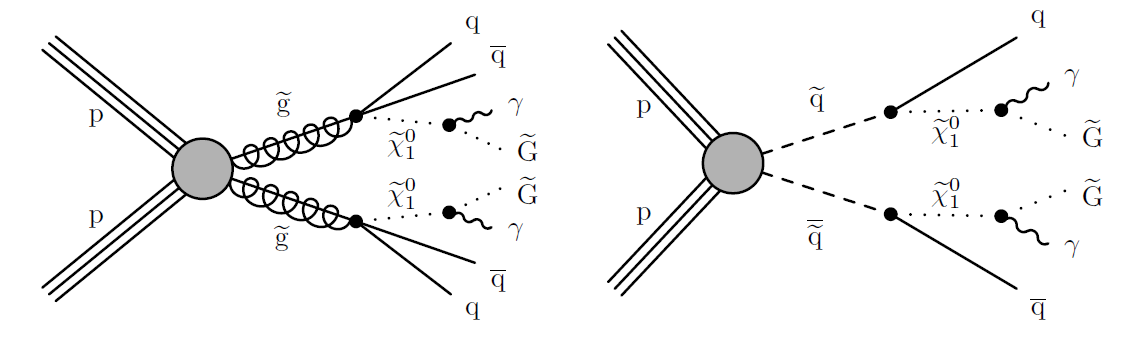
\includegraphics[width=0.9\linewidth]{Figures/SUSYsignals}
	\caption{Two examples of GGM supersymmetry breaking processes resulting in final states conaining two photons and missing transverse momentum. The T5gg model (left) shows gluinos produced from $p-p$ collisions which subsequently result in two neutralinos, each decaying to a photon and a gravitino. The T6gg model (right) shows squarks produced from $p-p$ collisions following a similar decay chain.}
	\label{fig:susysignals}
\end{figure}


\section{Data}
This analysis was performed using 137 fb$^{-1}$ of data collected from the CMS detector during the time period commonly referred to as Run 2 which spans from  2016 to 2018.  The complete list of the datasets used can be found in Table \ref{table:DataSamples}.  The JSON files used to identify events passing all of the CMS offline data quality monitoring requirements are:

\begin{verbatim}
	Cert_271036 284044_13TeV_23Sep2016ReReco_Collisions16_JSON.txt
	Cert_294927 306462_13TeV_EOY2017ReReco_Collisions17_JSON_v1.txt 
	Cert_314472 325175_13TeV_PromptReco_Collisions18_JSON.txt 
\end{verbatim} 

\begin{table}[h!]
	\centering
	\caption{Data Samples}
	\begin{tabular}{|c|}
		\hline
		/DoubleEG/Run2016B-17July2018-ver2-v1 \\
		\hline
		/DoubleEG/Run2016C-17July2018-v1 \\
		\hline
		/DoubleEG/Run2016D-17July2018-v1 \\
		\hline
		/DoubleEG/Run2016E-17July2018-v1 \\
		\hline
		/DoubleEG/Run2016F-17July2018-v1 \\
		\hline
		/DoubleEG/Run2016G-17July2018-v1 \\
		\hline
		/DoubleEG/Run2016H-17July2018-v1 \\
		\hline
		/DoubleEG/Run2017B-31Mar2018-v1 \\
		\hline
		/DoubleEG/Run2017C-31Mar2018-v1 \\
		\hline
		/DoubleEG/Run2017D-31Mar2018-v1 \\
		\hline
		/DoubleEG/Run2017E-31Mar2018-v1 \\
		\hline
		/DoubleEG/Run2017F-31Mar2018-v1 \\
		\hline
		/EGamma/Run2018A-17Sep2018-v2 \\
		\hline
		/EGamma/Run2018B-17Sep2018-v1 \\
		\hline
		/EGamma/Run2018C-17Sep2018-v1 \\
		\hline
	\end{tabular}
	\label{table:DataSamples}
\end{table}




\section{Monte Carlo samples}
Monte Carlo (MC) simulation were used to validate performance of the analysis on backgrounds, model background contributions, constructing a multivariate discriminant, and determining signal efficiencies.   


\section{Object definitions}
The object candidates that are identified by the reconstruction algorithms are subject to further scrutiny in order to achieve optimal purities in the offline analysis.  

\subsection{Photons}
Photons are required to have $p_T>75$ GeV and meet the criteria prescribed by loose ID cuts derived by the $e/\gamma$ Physics Object Group (EGM POG).  The cut variables used to determine the photon ID are:

\begin{itemize}
	\item H/E - The ratio of the energy deposited in the HCAL tower that is directly behind the ECAL supercluster associated with the photon to the energy deposited in the ECAL supercluster.
	\item $\sigma_{i\eta i\eta}$ - The log-fractional weighted width of a shower in $i\eta$-space.  This variable is used to describe the shower shape.
	\item Particle Flow Charged Isolation - Sum of the $p_T$ of charged hadrons associated with the primary vertex within a cone of $0.02 < \Delta R < 0.3$ of the supercluster.
	\item Particle Flow Neutral Isolation - Sum of the $p_T$ of neutral hadrons associated with the primary vertex within a cone of $\Delta R < 0.3$ of the supercluster.
	\item Particle Flow Photon Isolation - Sum of the $p_T$ of photons within a cone of $\Delta R < 0.3$ of the supercluster.
\end{itemize}

All of the isolation variables listed above are corrected in order to remove pileup.  Table \ref{table:looseIDPhotonreq} gives a summary of the pileup-corrected requirements for a loose ID photon.  The loose ID working point has an efficiency (background rejection) of $90.08\%$ ($86.25\%$) in the barrel and $90.65\%$ ($76.72\%$) in the end caps.  In addition to the $p_T$ and loose ID requirements, a photon must also pass a pixel seed veto (PSV).  This means that there is no pixel seed matched to the photon.

\begin{table}[h]
	\centering
	\caption{Summary of loose ID photons cuts}
	\begin{tabular}{|l|l|l|}
		\hline
		Variable & Cut Value (Barrel) & Cut Value (Endcap) \\
		\hline
		H/E & 0.04596 & 0.0590 \\
		\hline
		$\sigma_{i\eta i\eta}$ & 0.0106 & 0.0272 \\
		\hline
		Charged Iso & 1.694 & 2.089 \\
		\hline
		Neutral Iso & $24.032 + 0.01512 p_{T\gamma} + 2.259\times 10^{-5}p^2_{T\gamma}$ & $19.722 + 0.0117 p_{T\gamma} + 2.3\times 10^{-5}p^2_{T\gamma}$ \\
		\hline
		Photon Iso & $2.876 + 0.004017 p_{T\gamma}$ & $4.162 + 0.0037 p_{T\gamma}$ \\
		\hline
	\end{tabular}
	\label{table:looseIDPhotonreq}
\end{table}



\subsection{Electrons}
As mentioned earlier, the clustering algorithm doesn't differentiate between showers from photons and those from electrons.  In this analysis an electron is defined as an object that passes all of the photon requirements except for the PSV.  Inverting the pixel seed requirement while using the same ID criteria insures that we have orthogonal selections while minimizing the bias potentially introduced by using control regions with electrons to model diphoton signal regions. 


\subsection{Muons}

\section{Backgrounds}
The sources of background in this analysis can be grouped into three categories.  In order of decreasing contribution they are mismeasured hadronic activity, electrons misidentified as photons, and standard model processes having final states with neutrinos and two photons.  In events with multiple jets, limitations on the jet energy resolution can give rise to an apparent imbalance in $p_T$ as is shown in Figure \ref{fig:fakemet}.  Such events are usually from quantum chromodynamics (QCD) processes.  In these cases jets can be misidentified as photons or there can be real photons being produced.  In both cases the result is the appearance of two photons accompanied by $E^{miss}_T$ which mimics our signal.  Given the large cross-section for QCD, this is the most significant background in this analysis.  The next background, resulting from the misidentification of electrons as photons, comes from electroweak (EWK) processes, in particular $W\gamma$ and $W + jets$ events where $W \rightarrow e\nu$.  Here the neutrino contributes real $E^{miss}_T$ while the fake photon allows this event to fulfill the diphoton requirement.  The final background is from $Z\gamma \gamma \rightarrow \nu \nu \gamma \gamma$ events, which exactly mimic our signal, and is modeled using simulation as it is irreducible.

\begin{figure}
	\centering
	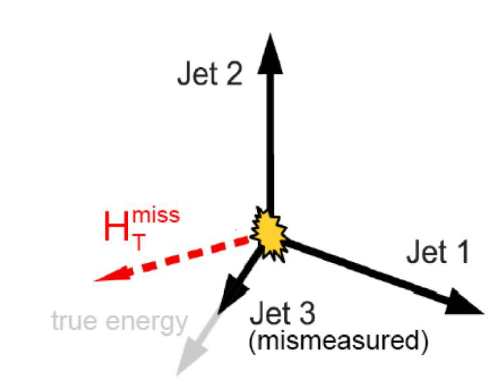
\includegraphics[width=0.5\linewidth]{Figures/FakeMET}
	\caption{Mismeasurement of Jet3 results in an inbalance in the events transverse momentum.}
	\label{fig:fakemet}
\end{figure}

\subsection{Instrumental background}
The instrumental background is the contribution from events with spurious $E^{miss}_T$ due to mismeasured hadronic activity.  Since most of this background is comprised of QCD events, it is commonly referred to as the "QCD background" and those terms are used interchangeably in this thesis.  Modeling of this background was done using the Rebalance and Smear technique while an multivariate discriminant was constructed to improve the efficiency of identifying events with fake $E^{miss}_T$.

\subsubsection{Rebalance and smear}
The rebalance and smear method is used to estimate the QCD background by 
\subsubsection{Multivariate discriminant}

\subsection{Electroweak background}
Need to look at this again

The electroweak background is dominated by events with $W \rightarrow e \nu$ where the electron is misidentified as a photon.  Unlike the QCD background these events have  real $E^{miss}_T$ due to the presence of a neutrino.  The key to estimating this background is determining the rate at which electrons get incorrectly labeled as photons in the signal region.  This is done using a tag-and-probe method where the tag is an electron (a loose ID photon that fails the PSV) and the probe is categorized as either a photon or an electron.  The result is an electron-electron region ($ee$) and an electron-photon region ($e\gamma$) that are selected from the data.    As both of these regions contain $Z\rightarrow ee$ decays, fits are applied in each of the samples to the invariant mass spectra $m_{ee}$ and $m_{e\gamma}$.  The integrals of these fits are calculated over the range of the Z mass peak to give 


This is done using two control regions.  The first is double electron ($ee$) region.  As described before, the electrons are defined as loose ID photons that have a pixel seed match.  The second is the $e\gamma$ region which contains one electron and one photon.  The misidentification rate can be calculated by comparing the invariant mass peaks $m_{ee}$ and $m_{e\gamma}$.  



\subsection{Irreducible background}
The irreducible $Z \gamma \gamma \rightarrow \nu \nu \gamma \gamma$ background produces two photons and has inherent $E^{miss}_T$ via the neutrinos.  There is no easy way to separate these events from our signal so it is estimated using MC simulation.  The modeling of this background was tested using $Z\gamma \gamma \rightarrow \mu \mu \gamma \gamma$ events in data.  Dimuon events with $|m_{\mu \mu} - m_Z|<10$ GeV were selected and the contribution of the muons was removed from the $E^{miss}_T$ calculation to mimic $Z\rightarrow \nu \nu$.